\documentclass{article}
\usepackage{graphicx}

\begin{document}
	\title{Data Science Coding Challenge: Twitter Sentiment Analysis}
	\author{Vasco Fernandes}
	\maketitle
	\tableofcontents
	\section{Introduction}
		Hate  speech  is  an  unfortunately  common  occurrence  on  the  Internet.  Often social media sites like Facebook and Twitter face the problem of identifying and censoring  problematic  posts  while weighing the right to freedom of speech. The  importance  of  detecting  and  moderating hate  speech  is  evident  from  the  strong  connection between hate speech and actual hate crimes. 
		
		Early identification of users promoting  hate  speech  could  enable  outreach  programs that attempt to prevent an escalation from speech to action. Sites such as Twitter and Facebook have been seeking  to  actively  combat  hate  speech. In spite of these reasons, NLP research on hate speech has been very limited, primarily due to the lack of a general definition of hate speech, an analysis of its demographic influences, and an investigation of the most effective features.
	\section{Problem Statement}
		The objective of this project is to find the best classification model to classify tweets.
		
		The objective of this task is to detect hate speech in tweets. For the sake of simplicity, we say a tweet contains hate speech if it has a racist or sexist sentiment associated with it. So, the task is to classify racist or sexist tweets from other tweets.
		
		Formally, given a training sample of tweets and labels, where label '1' denotes the tweet is racist/sexist and label '0' denotes the tweet is not racist/sexist, your objective is to predict the labels on the test dataset. 
		
	\section{Data Set}
	
	\subsection{Train Set}
	
	The data set provided (https://datahack.analyticsvidhya.com/contest/practice-problem-twitter-sentiment-analysis/) is composed by two different files, the train set ("$train\_E6oV3lV.csv$") and test set ("$test\_tweets\_anuFYb8.csv$"). The first file is composed by 31621 observations, with 3 columns ("id", "label" and "tweet"), with an uneven label (or class) distribution, as can be seen in Figure 1:
	
	\begin{figure}[h]
		\label{Figure 1}
		\caption{Class distribution}
		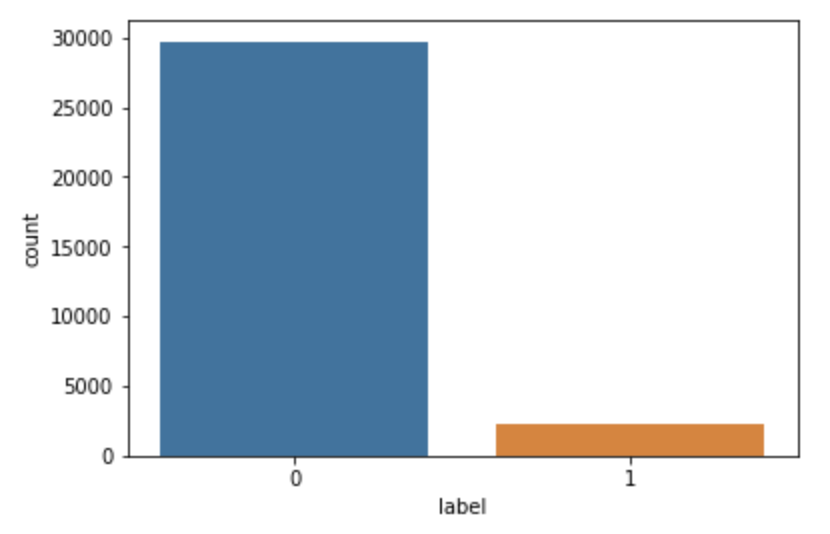
\includegraphics[width=9cm]{classes.png}
		\centering
	\end{figure}
	
	\subsection{Test Set}
	
	The test set is composed by 17197 observations, with only two columns ("id" and "tweet"). Given that this challenge is an open challenge, makes sense no "label" column, to make users submit their results. 
	
	\section{Initial Feature Engineering}
	
	\subsection{Pre-clean Tweet length}
	
	Given that in NLP tasks the most difficult challenge is the feature engineering part, and after applying algorithms out-of-box \textbf{after} cleaning and I was not able to produce good results, I tried to create my own features. 
	
	So the first hypothesis that I wanted to test was if one class of tweets has a statistically different pre-clean length that the other one. As we can see in Figure 2:
	
	\begin{figure}[h]
		\label{Figure 1}
		\caption{Pre-clean length}
		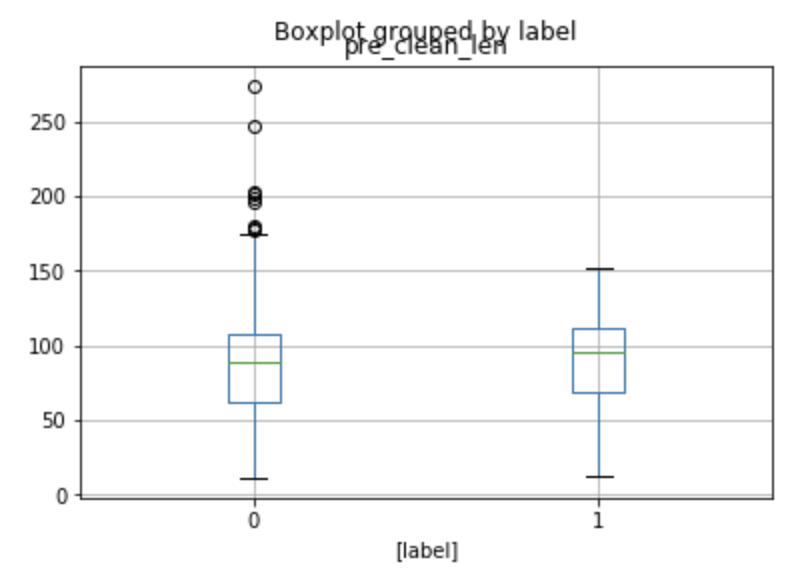
\includegraphics[width=9cm]{precleanl.png}
		\centering
	\end{figure}
	
	So, in terms of the median value, there is not a significant difference, but the $75^{th}$ percentile is somewhat deviated in class 0, comparing to class 1.  
	
	\subsection{Number of exclamation marks}
	
	So following the same line of thought of the last subsection, I thought that exclamation marks could be a discriminative feature. The hypothesis was that hate-speech tweets had more exclamation marks than non-hate speech tweets. The boxplot for each class in terms of the number of number of exclamation points. 
	
	\begin{figure}[!h]
		\label{Figure 1}
		\caption{Number of Exclamation Marks}
		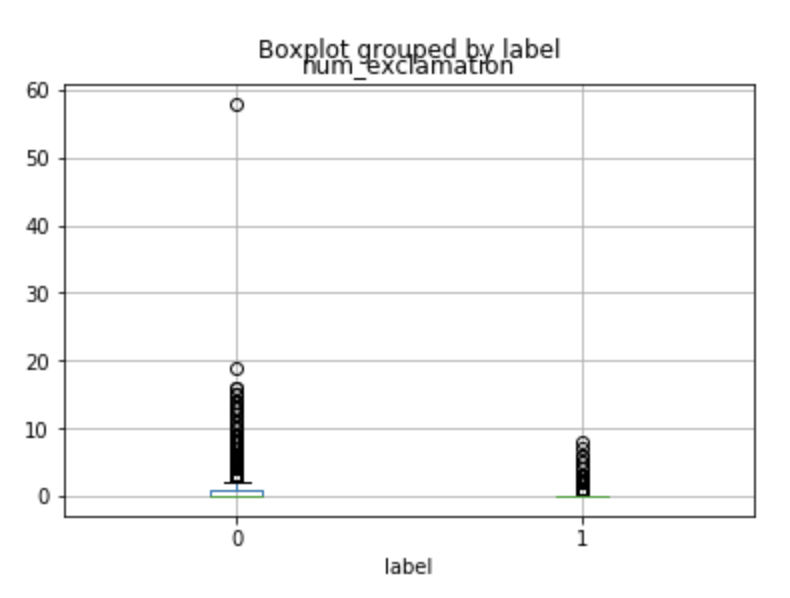
\includegraphics[width=9cm]{postcleanlength.png}
		\centering
	\end{figure}
	
	efwefwef
	
	\section{Data Cleaning}
	\section{Exploratory Data Analysis}
	\section{Algorithms \& Feature Engineering}
	\subsection{Logistic Regression}
	\subsection{Algorithm Comparison}
	\subsection{Deep Learning}
	\section{Discussion and Future Work}
\end{document}